%%%%%%%%%%%%%%%%%%%%%%%%%%%%%%%%%%%%%%%%%%%%%%%%%%%%%%%%%%%%%%%%%%%%%%
% This NoteBook is using Springer monograph template.
% This .tex file is coded in utf-8
% It is recomanded to compile this .tex file using XeLaTeX
% Anything confused by this file, you can contact me on github.com
% Good Luck, Have Fun.
%%%%%%%%%%%%%%%%%%%%%%%%%%%%%%%%%%%%%%%%%%%%%%%%%%%%%%%%%%%%%%%%%%%%%%

\documentclass[envcountsame,envcountchap]{svmono}

\usepackage{makeidx}              % allows index generation
\usepackage{graphicx}             % standard LaTeX graphics tool when including figure files
\usepackage{multicol}             % used for the two-column index
\usepackage[bottom]{footmisc}     % places footnotes at page bottom
\usepackage{xeCJK}                % Chinese support
\setCJKmainfont{等线}             % 中文字体设置
\setmainfont{Cambria}             % set English font
\usepackage{amsmath}
\usepackage{amsfonts}
\usepackage{fullpage}
\usepackage{indentfirst}          % 首行缩进
 \setlength{\parindent}{2em}
\usepackage{enumitem}
\usepackage{tikz}                 % draw some pictures
\usepackage{subfigure}
% etc.

\setcounter{chapter}{-1}          % chapter 0

\makeindex             % used for the subject index
% please use the style svind.ist with
% your makeindex program


%%%%%%%%%%%%%%%%%%%%%%%%%%%%%%%%%%%%%%%%%%%%%%%%%%%%%%%%%%%%%%%%%%%%%%

\begin{document}
	
	\title{Theoretical Physics in One Month\\
	\small{Lectured by Tongzhe}}
	%\subtitle
	\maketitle
	
	\frontmatter%%%%%%%%%%%%%%%%%%%%%%%%%%%%%%%%%%%%%%%%%%%%%%%%%%%%%%
	
	%%%%%%%%%%%%%%%%%%%%%%%%%%%%%%%%%%%%%%%%%%%%%%%%%%%%%%%%%%%%%%%%%%%%%%
% 
% This .tex file is coded in utf-8
% 
%%%%%%%%%%%%%%%%%%%%%%%%%%%%%%%%%%%%%%%%%%%%%%%%%%%%%%%%%%%%%%%%%%%%%%
\thispagestyle{empty}
\vspace*{3.5cm}
\begin{flushright}

% write dedication here
{\large TO ALL PHYSICS LOVERS}

\end{flushright}
	%%%%%%%%%%%%%%%%%%%%%%%%%%%%%%%%%%%%%%%%%%%%%%%%%%%%%%%%%%%%%%%%%%%%%%
% 
% This .tex file is coded in utf-8
% 
%%%%%%%%%%%%%%%%%%%%%%%%%%%%%%%%%%%%%%%%%%%%%%%%%%%%%%%%%%%%%%%%%%%%%%
\preface

%% write preface here


%% sign here if you contribute to this NoteBook.
\vspace{1cm}
\begin{flushleft}\noindent
China,\hfill {\it Sean Zhang}\\
January 2017 \\
\end{flushleft}
	
	\tableofcontents
	
	
	\mainmatter%%%%%%%%%%%%%%%%%%%%%%%%%%%%%%%%%%%%%%%%%%%%%%%%%%%%%%%

	\chapter{导论}
\label{intro}

No pain, no gain.

\section{生而为人关心整个宇宙}

形而上学$\Leftrightarrow$metaphysics

\section{数学与物理}

\subsubsection{数学}
某个公理的集合$A\Rightarrow$很多有趣的结论$A^\prime$。数学即“$\Rightarrow$”:严密的推导过程,但并不关心$A$与$A^\prime$的真实性。例如欧式几何与非欧几何。

\subsubsection{物理}
物理有实验作为标准。物理的关心基本假设(公理)$A$的正确性,通过数学的严密的推导可以我们可以将$A$的正确性传递给$A^\prime$,而通过实验验证$A^\prime$中的结论,我们也可以反过来验证我们的基本假设$A$的正确性。“可证伪性”。


数学研究的是某一个宇宙,物理研究的是我们的宇宙。

\section{所需的数学工具}

-高等数学

-线性代数

-复变函数

-群论

-点集拓扑

-特殊函数

-微分方程

-张量分析

-微分几何

\section{理论物理的框架}

\begin{tikzpicture}
	\node[shape=rectangle](a) at (0,0) {中学物理+普通物理(力、热、光、电、原子)};
	\node[shape=rectangle](b) at (0,-1.5){-理论力学};
	\node[shape=rectangle](c) at (0,-1.92){-热力学与统计物理};
	\node[shape=rectangle](d) at (0,-2.34){-电动力学};
	\node[shape=rectangle](e) at (0,-2.76){-量子力学};
	\node[shape=rectangle](f) at (0,-3.18){-广义相对论};
	\node[shape=rectangle](g) at (3,-2.55){量子电动力学};
	\node[shape=rectangle](h) at (3,-2.97){量子引力};
	\node[shape=rectangle](i) at (0,-3.6){etc...};
	\node[shape=rectangle,color=red](j) at (-2.5,-2.34){理论物理基础};
	\draw[->] (a) -- node[color=red,pos=0.25,left=33]{基础物理}(b);
	\draw[->] (d) -- (1.9,-2.55);
	\draw[->] (e) -- (1.9,-2.55);
	\draw[->] (e) -- (2.2,-2.97);
	\draw[->] (f) -- (2.2,-2.97);
\end{tikzpicture}

动态更新:
\begin{enumerate}[fullwidth,itemindent=2em,label=(\arabic*)]
	\item 光子的Bose-Einstein凝聚。\\
	\item 引力是一种熵力。\\
	\item 火墙。\\
\end{enumerate}

\section{先修知识}

\[f^\prime(x), \quad \int e^x \dd x  = e^x+C, \quad \log^\prime x = \frac{1}{x}, \quad \epsilon-\delta\text{语言}\]

\subsubsection{6个初等函数}
\begin{enumerate}[fullwidth,itemindent=2em,label=(\arabic*)]
	\item 常函数:$f(x) = C$\\
	\item 幂函数:$f(x) = x^a (a \neq 0)$\\
	\item 指数函数:$f(x) = a^x (a > 0)$\\
	\item 对数函数:$f(x) = \log_a x$\\
	\item 三角函数:$\sin x, \ \cos x, \ \tan x, \ \cot x$\\
	\item 反三角函数:$\arcsin x, \ \arccos x, \ \arctan x$ 
\end{enumerate}

双曲余弦:
\[\cosh x \equiv \frac{e^x+e^{-x}}{2}\]
对应$\leftrightarrow$余弦函数:
\[\cos x \equiv \frac{e^{ix}+e^{-ix}}{2}\]

\subsubsection{Taylor展开}
\begin{equation}
f(x) = f(0)+f^\prime(0)x+\frac{f^{\prime\prime}(0)}{2!}x^2+...+\frac{f^{(n)}(x)}{n!}x^n+...
\end{equation}
回忆匀变速直线运动公式:$x = x_0+vt+\frac{a}{2}t^2$

\subsubsection{分部积分}
\begin{equation}
\int_{x_1}^{x_2} f^\prime(x)g(x)\dd x = \left.f(x)g(x)\right|_{x_1}^{x_2} - \int_{x_1}^{x_2} f(x)g^\prime(x)\dd x
\end{equation}

\begin{figure}
	\centering
	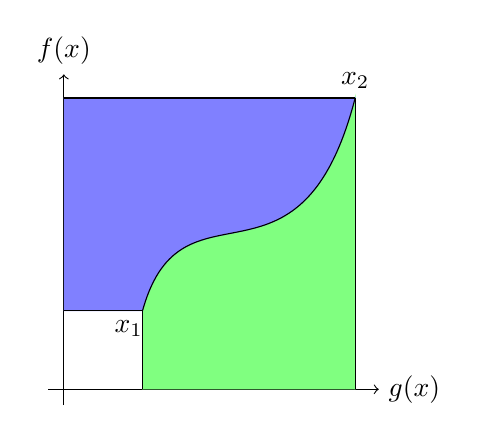
\begin{tikzpicture}
		\draw[->] (-0.2,0) -- (4,0) node[right]{$g(x)$};
		\draw[->] (0,-0.2) -- (0,4) node[above]{$f(x)$};
		\node[left=5,below](x1) at (1,1) {$x_1$};
		\node[right,above](x2) at (3.7,3.7) {$x_2$};
		\filldraw[green!50] (1,0) -- (1,1) ..controls(1.5,2.8) and (3,1) ..(3.7,3.7) -- (3.7,0);
		\filldraw[blue!50] (0,1) -- (1,1) ..controls(1.5,2.8) and (3,1) ..(3.7,3.7) -- (0,3.7);
		\draw (1,1) ..controls(1.5,2.8) and (3,1) ..(3.7,3.7);
		\draw (1,0) -- (1,1);
		\draw (0,1) -- (1,1);
		\draw (3.7,3.7) -- (3.7,0);
		\draw (3.7,3.7) -- (0,3.7);
	\end{tikzpicture} 
	\caption{分部积分示意图}
\end{figure}

\subsubsection{微分方程}
受迫阻尼振动:
\[m \ddot{x} = -kx-\gamma \ddot{x}+F(t)\]
Schrödinger方程:
\[i\hbar \frac{\partial \psi}{\partial t} = -\frac{\hbar^2}{2m} \frac{\partial^2 \psi}{\partial x^2}+V\psi\]

\subsubsection{卷积}
\begin{align}
k(t) = \int_{x_1}^{x_2} f(x) g(t-x) \dd x  \equiv f*g\\
(f*g)*h = f*(g*h)
\end{align}

\subsubsection{高等数学中难理解的问题}
Q:$f(x)$在0点光滑,$f^{(n)} = 0$,Taylor展开之后:$f(x) = 0$?
\[
f(x) = \left\{
\begin{array}{lc}
e^{-\frac{1}{x^2}} & (x \neq 0)\\
0                  & (x = 0)     
\end{array}
\right.
\]

\begin{figure}
	\centering
	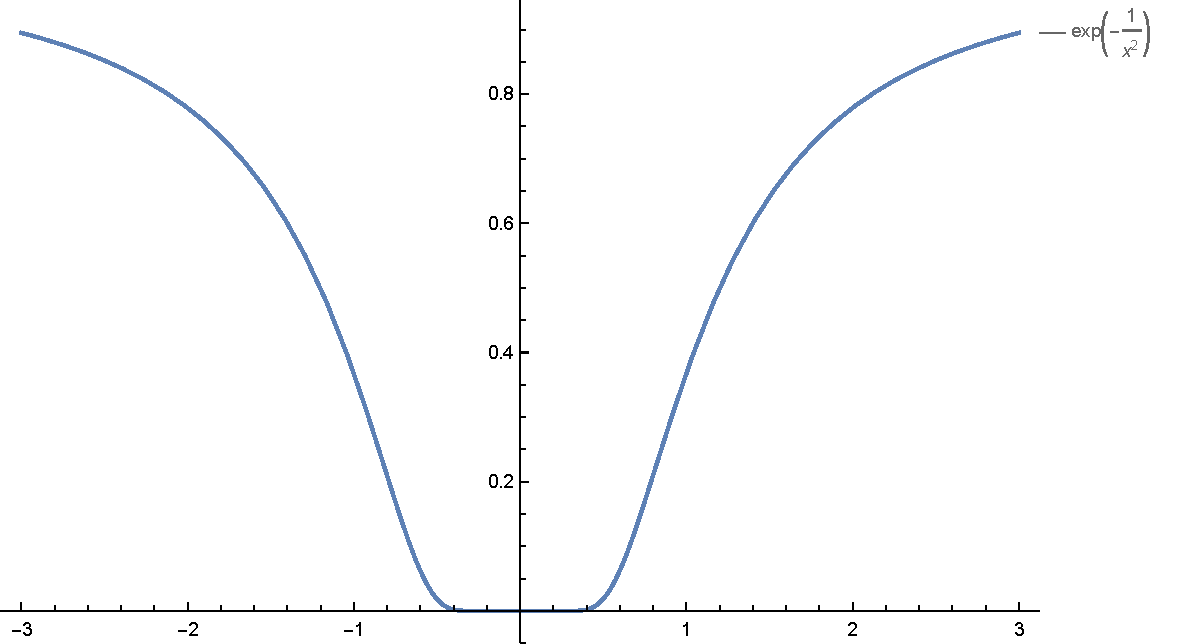
\includegraphics[width=14cm]{Figures/Exp[-x^-2].pdf}
	\caption{\(f(x)\)图像}
\end{figure}

A:在复变函数中
\[f(z)=e^{-\frac{1}{z^2}}\]
在$z = 0$有本性奇点,展开半径为0,故不能Taylor展开,但可以用Laurent展开。

Q:为何函数
\[g(x)=\frac{1}{1+x^2}\]
Taylor展开的收敛区域为$(-1,1)$?

A:在复数域看:$g(z)=\frac{1}{1+z^2}$在$\pm i$为奇点!所以展开半径为1,只能在$(-1,1)$展开。





	
	%%%%%%%%%%%%%%%%%%%%%%%%%%%%%%%%%%%%%%%%%%%%%%%%%%%%%%%%%%%%%%%%%%%%%%
% 
% This .tex file is coded in utf-8
% 
%%%%%%%%%%%%%%%%%%%%%%%%%%%%%%%%%%%%%%%%%%%%%%%%%%%%%%%%%%%%%%%%%%%%%%
\part{数学基础}
	%%%%%%%%%%%%%%%%%%%%%%%%%%%%%%%%%%%%%%%%%%%%%%%%%%%%%%%%%%%%%%%%%%%%%%
% 
% This .tex file is coded in utf-8
% 
%%%%%%%%%%%%%%%%%%%%%%%%%%%%%%%%%%%%%%%%%%%%%%%%%%%%%%%%%%%%%%%%%%%%%%
\chapter{数学大冒险}
\label{Chap1}
% Always give a unique label
% use \chaptermark{}
% to alter or adjust the chapter heading in the running head

物理是巧妙的要求自己。“费曼估算”

对一般物理学家,误差在$5\%$以内便可以接受。粒子物理学家误差$10^{-6}$;天体物理学家,相同数量级。

“实用主义”

\section{实数}
\label{ss}
% Always give a unique label
% and use \ref{<label>} for cross-references
% and \cite{<label>} for bibliographic references
% use \sectionmark{}
% to alter or adjust the section heading in the running head

为什么需要实数?

有理数$p/q, p,q\in \mathbb{Z}$。$\pi$是一个无理数,可以用有理数来逼近,但最后极限却不是有理数:
\[3,\ 3.1,\ 3.14,\ 3.141,\ ...\]
有理数完备化$\rightarrow$实数。“戴德金分划”

\subsection{戴德金分划}
\label{ddjfh}

有理数的定义:$\mathbb{Q} = \{p/q|\ p,q\in \mathbb{Z}\}$。有理数和无理数都很稠密:任一区间都有无穷多的有理数和无理数。

戴德金分划:将有理数切开:
\begin{enumerate}[fullwidth,itemindent=2em]
	\item $\mathbb{Q} = A_1\cup A_2$
	\item $A_1\cap A_2 = \emptyset$
	\item $\forall a_1\in A_1, \forall a_2\in A_2, a_1 < a_2$
\end{enumerate}

这种有理数的分割有三种可能:
\begin{enumerate}[fullwidth,itemindent=2em,label=(\arabic*)]
	\item 在下组$A_1$内无最大数,而在上组$A_2$内有最小数$r$
	\item 在下组$A_1$内有最大数$r$,而在上组$A_2$内无最小数
	\item 在下组$A_1$内既无最大数,在上组$A_2$内也无最小数
\end{enumerate}
前两种分划称为有理分划,最后一种称为无理分划。由分划可以定义实数:下组$A_1$的上确界。

由此还可以定义实数的大小:$\mathbb{Q} = A_1\cup A_2 = A_1^\prime\cup A_2^\prime$,若$A_1\subset A_1^\prime$,那么$A_1$所定义的实数要小于$A_1^\prime$所定义的实数。

天生的保证实数具有完备性,再进行分划不能再进行有意义的扩张。

“完备性”$\Rightarrow$ 单调有界序列在$\mathbb{R}$中存在极限。

\subsection{有理数集和实数集“大小”的比较}
\label{ylsjhshjdxdbj}

“希尔伯特的旅馆”

集合的“势”的比较。“势”$\Leftrightarrow$集合元素的个数。

定义:集合元素个数相同:存在两个集合间的一一对应。

\subsubsection{有理数与自然数}

有理数集$\mathbb{Q} = \{\frac{p}{q}\ |p,q\in \mathbb{Z},q>0\}$。可以由$|p|+|q|$由小到大一一编号。即$\mathbb{Q}$与$\mathbb{N}$元素个数相同。

$\mathbb{Q},\mathbb{N}, \mathbb{Z}$元素个数相同,$\aleph_{0}$个 

\subsubsection{实数个数远超有理数个数}

$(0,1)$内实数可以表示为:$k=0.a_{1}a_{2}a_{3}a_{4}a_{5}...$

“反证法”:假设存在$(0,1)$内的所有实数与正整数一一对应。
\begin{align*}
1\leftrightarrow0.&a_{1}a_{2}a_{3}a_{4}a_{5}...\\
2\leftrightarrow0.&b_{1}b_{2}b_{3}b_{4}b_{5}...\\
3\leftrightarrow0.&c_{1}c_{2}c_{3}c_{4}c_{5}...\\
&...
\end{align*}

欲构造某个实数$k$不在该序列中。

先构造:$k^\prime = 0.a_{1}b_{2}c_{3}d_{4}e_{5}...$,存在某个自然数$n_0\leftrightarrow k^\prime$。有$k^\prime$构造$k$:每一位若非9,则变为9,若为9,则变为0。若$N_1\leftrightarrow k$,那么$N_1$位上$k$与$k^\prime$在$N_1$位上必为相同数字$\omega$!矛盾!故所有实数与正整数不一一对应。

$\mathbb{R}$的元素个数:$\aleph_1$。

可以证明二维平面上$(0,1)\times(0,1)$上的某点可以和一维实轴上的某点一一对应:
\[(0.a_{1}a_{2}a_{3}a_{4}a_{5}...,0.b_{1}b_{2}b_{3}b_{4}b_{5}...)\leftrightarrow0.a_{1}b_{1}a_{2}b_{2}a_{3}b_{3}a_{4}b_{4}a_{5}b_{5}...\]

$\mathbb{R}^n$的元素个数:$\aleph_1$。

$\aleph_2?\Rightarrow(0,1)$区间内实函数的个数。

\subsection{一点点测度论"a little bite of Measure Theory"}
\label{yddcdl}

为何$\mathbb{R}$元素个数远多于$\mathbb{Q}$?

测度(measure):衡量一个区间、集合有多“长”。$A$为集合,则:
\[M(A)\rightarrow\mathbb{R}\]

常规结论:

\begin{enumerate}[fullwidth,itemindent=2em]
	\item $M{(a,b)} = b-a$
	\item 若$A\subset A^\prime$,则$M(A) \ge M(A^\prime) \ge 0$
	\item $M(\emptyset) = 0$
\end{enumerate}

求证:
\begin{equation}
M(\mathbb{R})\rightarrow \infty,\ M(\mathbb{Q}=0)
\end{equation}

证明:$M(\mathbb{R}\rightarrow \infty)$是平凡的。

$\mathbb{Q}$与$\mathbb{N}$是一一对应的,则$\mathbb{Q}$是可列的。\\
\[\mathbb{Q}=\{q_1,q_2,q_3,q_4,...\}\]
以$q_i$为中心构造一个开区间包住$q_i$,$A_i \equiv (q_i-\frac{\epsilon}{2^i},q_i+\frac{\epsilon}{2^i})$,${q_i\subset A_i}$

将所有的$A_i$集合求全集$A = \cup_{i=1}^{+\infty}A_i$,因为${q_i \subset A_i}$,所以$\mathbb{Q}\subset A$,所以
\[0 \le M(\mathbb{Q}) \le M(A)\]
又:
\[M(A) \le \sum_{i=1}^{\infty}M(A_i) = \sum_{i=1}^{\infty}[(q_i+\frac{\epsilon}{2^i})-(q_i-\frac{\epsilon}{2^i})] = \sum_{i=1}^{\infty}2\frac{\epsilon}{2^i}=2\epsilon\]
即:
\[0 \le M(\mathbb{Q}) \le M(A) \le 2\epsilon\]
因为$\forall \epsilon >0$,所以取$\epsilon \rightarrow 0$,所以$M(\mathbb{Q})=0$

\section{无穷大量的排序}
\label{wqdldpx}

$n \in \mathbb{N},\ x \in \mathbb{R};\ n \rightarrow +\infty$

常见无穷大量:$n^6,\sqrt{n},n^n,n!,\log n$,有无穷大量排序\\
\begin{equation}
\log n \ll n^{\frac{1}{a_1}} \ll n \ll n^{a_2} \ll a_3^{n} \ll n! \ll n^n \ \ (a_1,a_2,a_3>1)
\end{equation}

求证:$\lim\limits_{n \rightarrow \infty} \frac{n^{a_2}}{a_3^n}=0$

证明: 将$a_3^n$展开成幂级数,次数大于$a_2$\\
令$h = a_3-1>0$,有:\\
\[a_3^n = (1+h)^n = 1+nh+\frac{n(n-1)}{2!}h^2+\frac{n(n-1)(n-2)}{3!}h^3+...+\frac{n(n-1)...(n-k)}{(k+1)!}h^{k+1}+...+h^n\]
其中$k = [a_2]+1>a_2$。因为:\\
\[0 \le \frac{n^{a_2}}{a_3^n} \le \frac{n^k}{\frac{n(n-1)...(n-k)}{(k+1)!}h^{k+1}} = \left[\frac{(k+1)!}{h^{k+1}}\right]\left(\frac{1}{n}\right)\left(\frac{n}{n-1}\right)\left(\frac{n}{n-1}\right)...\left(\frac{n}{n-k}\right)\]
取$n\rightarrow\infty$,根据夹逼定理,有:
\[\lim\limits_{n \rightarrow \infty} \frac{n^{a_2}}{a_3^n}=0\]

求证:$\lim\limits_{n \rightarrow \infty} \frac{a^n}{n!} = 0$

证明:取$N=[a]+1$,有:

\[0 \le \frac{a^n}{n!} \le \frac{a\cdot a\cdot ...a}{1\cdot 2\cdot ...N}\cdot\left(\frac{a}{n-N}\right)^{n-N}\]

因为$n\rightarrow\infty$时,$(n-N)\rightarrow\infty$,所以$\frac{a}{n-N}<1$,那么$\left(\frac{a}{n-N}\right)^{n-N}\rightarrow0$,即:

\[0 \le \lim\limits_{n \rightarrow \infty} \frac{a^n}{n!} \le \lim\limits_{n \rightarrow \infty}[C\cdot\left(\frac{a}{n-N}\right)^{n-N}] = 0\]

由无穷大量排序可得无穷小量的排序:
\begin{equation}
\frac{1}{\log n} \gg \frac{1}{n^{\frac{1}{a_1}}} \gg \frac{1}{n} \gg \frac{1}{n^{a_2}} \gg \frac{1}{a_3^{n}} \gg \frac{1}{n!} \gg \frac{1}{n^n} \ \ (a_1,a_2,a_3>1)
\end{equation}
\subsubsection{收敛的边界}
\[S_n=\sum_{i=1}^{n}a_i\]
何时$S_n$有极限?
\begin{equation}
\left. \frac{1}{\log n} \gg \frac{1}{n^{\frac{1}{a_1}}} \gg \frac{1}{n} \right|\gg \frac{1}{n^{a_2}} \gg \frac{1}{a_3^{n}} \gg \frac{1}{n!} \gg \frac{1}{n^n} \ \ (a_1,a_2,a_3>1)
\end{equation}
在求和时竖线右侧的会收敛,左侧则发散。

求证:若$a>1$,则$\sum_{n=1}^{+\infty}\frac{1}{n^a}$收敛。

证明:每$2^n$项一组$n=0,1,2...$:
\[\sum_{n=1}^{+\infty}\frac{1}{n^a} = \left(\frac{1}{1^a}\right)+\left(\frac{1}{2^a}+\frac{1}{3^a}\right)+\left(\frac{1}{4^a}+\frac{1}{5^a}+\frac{1}{6^a}+\frac{1}{7^a}\right)+\frac{1}{8^a}+... \le \frac{1}{1^a}+2\cdot\frac{1}{2^a}+...+2^n\cdot\frac{1}{2^{na}}+... = \sum_{n=0}^{+\infty} \frac{1}{2^{n(a-1)}}\]
所以:
\[\sum_{n=1}^{+\infty}\frac{1}{n^a} \le \frac{1}{1-\frac{1}{2^{a-1}}} = \frac{2^{a-1}}{2^{a-1}-1} = constant\]
即:$\sum_{n=1}^{+\infty}\frac{1}{n^a}$收敛。

\subsubsection{更细的收敛边界}

\begin{equation}
\left.\frac{1}{n} > \frac{1}{n\log n} \right| > \frac{1}{n(\log n)^{a_1}} > \frac{1}{n^{a_2}}  \ \ (a_1,a_2>1)
\end{equation}
更细?
\begin{equation}
\left. \frac{1}{n\log n \log (\log n)} \right| > \frac{1}{n\log n (\log (\log n))^a} \ \ (a>1)
\end{equation}

\subsubsection{有趣的未定收敛的例子}

规整级数,初等函数$\rightarrow \_ \rightarrow$
\[a_n=\frac{1}{n^2 \sin n}\],\[S=\sum_{n=1}^{\infty}a_n\] 未定收敛,其收敛性与$\pi$的无理测度有关。

无理测度$\mu(x)$
\[\mu(x)\left\{ 
	\begin{array}{ll}
	1  \  &   ,\ x\text{有理数}\\
	2  \  &   ,\ \text{代数数阶>1的无理数}\\
	>2 \  &   ,\ \text{超越数}
	\end{array}
\right.\]
已知$\mu(\pi)<7.6063$,若$\mu(\pi)<3$,则$a_n$收敛。

\section{级数求和}
\label{jsqh}

\subsection{一般的级数}

\begin{enumerate}
	\item 
		利用Taylor展开:\\
		利用$\log (1+x)$在$x=0$的Taylor展开:
		\begin{equation}
		1-\frac{1}{2}+\frac{1}{3}-\frac{1}{4}+\frac{1}{5}+... = \log 2
		\end{equation}
		利用$e^x$在$x=0$处的Taylor展开:
		\begin{equation}
		1+\frac{1}{1!}+\frac{1}{2!}+\frac{1}{3!}+\frac{1}{4!}+... = e
		\end{equation}
	\item 利用Fourier级数:
		\begin{equation}
		f(x) = \frac{1}{2}a_0+\sum_{n=1}^{+\infty}a_n \cos nx+\sum_{n=1}^{+\infty}b_n \sin nx
		\end{equation}
		Fourier级数在中断点取中间值。
		\[1-\frac{1}{3}+\frac{1}{5}-\frac{1}{7}+\frac{1}{9}-... = ?\]
		构造:
		\[f(x) = \left\{
		\begin{array}{ll}
		0 &\ \ \  ,         -\pi < x < 0\\
		1 &\ \ \  ,            0 < x < \frac{\pi}{2}\\
		0 &\ \ \  ,\frac{\pi}{2} < x < \pi
		\end{array}
		\right.\]
		且其周期为$2\pi$,可知它的Fourier展开为:
	    \[
	    \begin{split}
	    f(x) =& \frac{1}{4} + \frac{1}{\pi} \sum_{n=1}^{+\infty} \frac{\sin \left(\frac{n\pi}{2}\right)}{n} \cos nx + \frac{1}{\pi} \sum_{n=1}^{+\infty} \frac{2 \sin ^2\left(\frac{n\pi}{4}\right)}{n} \sin nx\\
	    =& \frac{1}{4}+\frac{1}{\pi}\left(\frac{\cos x}{1}-\frac{\cos 3x}{3}+\frac{\cos 5x}{5}-...\right)+\frac{1}{\pi}\left(\frac{\sin x}{1}+\frac{2 \sin 2x}{2}+\frac{\sin 3x}{3}+\frac{\sin 5x}{5}+...\right)
	    \end{split}
	    \]
	    取$x=0$,可以得到:
	    \begin{equation}
	    1-\frac{1}{3}+\frac{1}{5}-\frac{1}{7}+\frac{1}{9}-... = \frac{\pi}{4}
	    \end{equation}
    \item
	    利用Parseval定理(“勾股定理加强版”)\\
	    由Fourier级数我们有:
	    \[f(x) = \frac{1}{2}a_0+\sum_{n=1}^{+\infty}a_n \cos nx+\sum_{n=1}^{+\infty} b_n \sin nx\]
	    所以:
	    \begin{equation}
	    \left|f(x)\right|^2 = \left(\frac{a_0}{2}\right)^2+\sum_{n=1}^{+\infty}\frac{1}{2}a_n^2+\sum_{n=1}^{+\infty}\frac{1}{2}b_n^2
	    \end{equation}
	    其中:
	    \[\left|f(x)\right|^2 \equiv \int_L f^*(x)f(x)\mathrm{d}x\]
	    此即Parseval定理:\\
	    求解:
	    \[1+\frac{1}{2^2}+\frac{1}{3^2}+\frac{1}{4^2}+\frac{1}{5^2}+... = ?\]
	    解:考虑:
	    \[f(x) = x \ \ ,x\in(-1,1)\]
	    其周期为2,有Parseval定理可得:
	    \[
	    \begin{split}
	    \left|f(x)\right|^2 &= \int_{-1}^{1}x^2\mathrm{d}x = \frac{1}{3}\\
	                        &= \frac{2}{\pi^2} \sum_{n=1}^{+\infty}\frac{1}{n^2}
	    \end{split}
	    \]
	    所以:
	    \begin{equation}
	    \sum_{n=1}^{+\infty} \frac{1}{n^2} = 1+\frac{1}{2^2}+\frac{1}{3^2}+\frac{1}{4^2}+\frac{1}{5^2}+... = \frac{\pi^2}{6}
	    \end{equation}
\end{enumerate}

微小的改变将使得级数求和变得极为困难;很多级数求和本身就十分困难。$\rightarrow$数值求解会是我们最后的希望。

\subsection{交错级数}

交错级数的定义:交错级数是形如:
\[\sum_{n=0}^\infty (-1)^n\ a_n\]
的级数,其中$a_n \ge 0$。

\subsubsection{交错级数的一个审敛法(莱布尼兹判别法)}

若各项非负的数列$a_n$单调递减且趋于零,则级数
\[\sum_{n=0}^\infty (-1)^n\ a_n\]
收敛。

证明:考虑$S_{2n}$和$S_{2n+1}(n\in \mathbb{Z},n \ge 0)$,我们有:
\[S_{2n+1} = S_{2n}-a_{2n+1}\]
所以$S_{2n} > S_{2n+1}$,又:
\[S_{2(n+1)} = S_{2n}-a_{2n+1}+a_{2n+2}\]
所以$S_{2n}$单调递减有上确界,同理$S_{2n+1}$单调递增有下确界。所以由$S_{2n} > S_{2n+1}$知:$S_{2n}$单调递减有下确界,$S_{2n+1}$单调递增有上确界。所以可知:
\[\lim\limits_{n\rightarrow+\infty}S_{2n} = L^+\]
\[\lim\limits_{n\rightarrow+\infty}S_{2n+1} = L^-\]
又因为$n\rightarrow+\infty$时,$a_n\rightarrow0$,所以:
\[
\begin{split}
\lim\limits_{n\rightarrow+\infty}S_{2n+1} &= \lim\limits_{n\rightarrow+\infty}(S_{2n}-a_{2n+1})\\
&= \lim\limits_{n\rightarrow+\infty}S_{2n}-\lim\limits_{n\rightarrow+\infty}a_{2n+1}\\
&= \lim\limits_{n\rightarrow+\infty}S_{2n}
\end{split}\]
所以$L^-=L^+$,即:
\[\lim\limits_{n\rightarrow+\infty}S_{n} = L\]
此时级数具有极限。
\subsubsection{条件收敛与绝对收敛}

给定一个实数项无穷级数$A = \sum_{n} a_n$,如果它自身收敛于一个定值$C \in \mathbb{R}$:
\[ \sum_{n=1}^\infty a_n = C\]
但由每一项的绝对值构成的正项级数:$A_s = \sum_{n} | a_n |$不收敛,那么就称这个无穷级数$A = \sum_{n} a_n$是一个条件收敛的无穷级数。

若由每一项的绝对值构成的正项级数:$A_s = \sum_{n} | a_n |$收敛,那么就称这个无穷级数$A = \sum_{n} a_n$是一个绝对收敛的无穷级数。

考察级数:
\[1-\frac{1}{3}+\frac{1}{5}-\frac{1}{7}+\frac{1}{9}-... = \frac{\pi}{4}\]
\begin{figure}
	\centering
	\includegraphics[width=5cm]{Figures/sum.pdf}
	\caption{$S_n=\sum_{i=1}^{n}\frac{(-1)^{n+1}}{2n-1}$}
	\label{sumjc}
\end{figure}
通过调换顺序可使其收敛至任何值。级数和$1-\frac{1}{3}+\frac{1}{5}-\frac{1}{7}+\frac{1}{9}-...$是条件收敛的,需要注意到求和顺序。

\subsubsection{Riemann级数定理}
\begin{theorem}
	假设$\sum_{n=1}^\infty a_n$是一个条件收敛的无穷级数。对任意的一个实数$C$,都存在一种从自然数集合到自然数集合的排列$\sigma : \, \, n \mapsto \sigma (n)$,使得:
	\[\sum_{n=1}^\infty a_{\sigma (n)} = C\]
	此外,也存在另一种排列$\sigma' : \, \, n \mapsto \sigma' (n)$,使得:
	\[\sum_{n=1}^\infty a_{\sigma' (n)} = \infty\]
	类似地,也可以有办法使它的部分和趋于$-\infty$,或没有任何极限。
	
	反之,如果级数是绝对收敛的,那么无论怎样重排,它仍然会收敛到同一个值,也就是级数的和。
\end{theorem}


\subsubsection{交错级数收敛极为缓慢}

\[1-\frac{1}{2}+\frac{1}{3}-\frac{1}{4}+\frac{1}{5}+... = \log 2\]
收敛到0.001精确度需要5000项。

\[1-\frac{1}{\sqrt{2}}+\frac{1}{\sqrt{3}}-\frac{1}{\sqrt{4}}+\frac{1}{\sqrt{5}}+... = 0.6048986...\]
收敛到0.001精确度需要$10^6?$项。

即使是绝对收敛的单调级数:
\[1+\frac{1}{2^2}+\frac{1}{3^2}+\frac{1}{4^2}+\frac{1}{5^2}+... = \frac{\pi^2}{6}\]
收敛到0.001精确度需要$1000$项。

\subsection{Shanks Transformation}
\label{st}

如何加速:
\[1-\frac{1}{2}+\frac{1}{3}-\frac{1}{4}+\frac{1}{5}-\frac{1}{6}+...\]
其和的数值表如下:\\
\begin{table}
	\centering
	\begin{tabular}{c|c}
		$n$  &  $S_n$\\
		\hline
		1    & 1.000 000 0\\
		2    & 0.500 000 0\\
		3    & 0.833 333 3\\
		4    & 0.583 333 3\\
		5    & 0.783 333 3\\
		6    & 0.616 666 7\\
		$\cdot\cdot\cdot$  & $\cdot\cdot\cdot$ 
	\end{tabular}
	\caption{$S_n=\sum_{i=1}^{n}\frac{(-1)^{n+1}}{n}$}
\end{table}
其收敛图类似于图\ref{sumjc}。类似于“阻尼振荡”,回想力学中受迫阻尼振荡将使得振荡周期与受迫里周期相同,受迫阻尼振荡的运动方程为:
\[m \ddot{x} = -kx -\gamma \dot{x} +F_0 \cos\omega t\]
其解为:
\[x(t) = x_0(t) +x^*(t) \]
其中$ x_0(t)$为衰减项,将随时间趋近于0;$x^*(t)$为驱动项,具有形式:$x^* = A\cos(\omega t + \phi)$

启示我们:可以给级数附加驱动模型。令:
\[S_n = L +a b^n\]
其中$b<0$,且$|b|<1$,但我们真正关心的是$L$,想办法用$S_n$表示$L$。我们有:
\[S_n = L +a b^n\]
\[S_{n+1} = L +a b^{n+1}\]
\[S_{n-1} = L +a b^{n-1}\]
由此可以解得:
\[L = \frac{S_n^2-S_{n+1}S_{n-1}}{2S_n-S_{n+1}-S_{n-1}}\]
此即Shanks变换。

例1:
\[1-\frac{1}{2}+\frac{1}{3}-\frac{1}{4}+\frac{1}{5}-\frac{1}{6}+... = 0.6931472...\]
其$S_1=1,S_2=0.5,S_3=0.8333$,由此可以利用此即Shanks变换得到:
\[L = 0.700\]
精确度1\%!

利用Shanks变换我们可以得到下表:
\begin{table}
	\centering
	\begin{tabular}{c|c|c|c|c}
		   $n$   &    $S_n$    &     $L_n$     &  $L_n^{(2)}$  &  $L_n^{(3)}$  \\
	    	\hline
		    1    & 1.000 000 0 &               &               &               \\
		    2    & 0.500 000 0 &               &               &               \\
		    3    & 0.833 333 3 &  0.700 000 0  &               &               \\
		    4    & 0.583 333 3 &  0.690 476 2  &               &               \\
		    5    & 0.783 333 3 &  0.694 444 4  &  0.693 277 3  &               \\
		    6    & 0.616 666 7 &  0.692 424 2  &  0.693 105 8  &               \\
		    7    & 0.759 523 8 &  0.693 589 7  &  0.693 163 3  &  0.693 148 9  \\
	\end{tabular}
	\caption{Shanks变换例1}
\end{table}

更详细可以参考华盛顿大学的Carl Bender的<Advanced Mathematical Methods for Scientists and Engineers I: Asymptotic Methods and Perturbation Theory>(《高级数理方法》)

例2:
\[1-\frac{1}{\sqrt{2}}+\frac{1}{\sqrt{3}}-\frac{1}{\sqrt{4}}+\frac{1}{\sqrt{5}}+... = 0.6048986...\]
利用Shanks变换我们可以得到下表:
\begin{table}
	\centering
	\begin{tabular}{c|c|c|c|c}
		$n$   &    $S_n$    &     $L_n$     &  $L_n^{(2)}$  &  $L_n^{(3)}$  \\
		\hline
		1    & 1.000 000 0 &               &               &               \\
		2    & 0.292 893 2 &               &               &               \\
		3    & 0.870 243 5 &  0.610 730 5  &               &               \\
		4    & 0.370 243 5 &  0.602 294 5  &               &               \\
		5    & 0.817 457 1 &  0.606 311 5  &  0.605 015 6  &               \\
		6    & 0.409 208 8 &  0.604 035 3  &  0.604 858 5  &               \\
		7    & 0.787 173 3 &  0.605 470 4  &  0.604 915 5  &  0.604 900 3  \\
	\end{tabular}
	\caption{Shanks变换例2}
\end{table}

由此我们可以感受到,多次Shanks变换可以大大加快级数收敛的速度。

\subsection{Richardson Extrapolation}
\label{re}

单调收敛级数,例如:
\[a_n=\frac{1}{n^2},\ \ S=\sum_{n=1}^{\infty}a_n=\frac{\pi^2}{6}\]

模型:
\begin{align}
&S_N \equiv \sum_{i=1}^{N}a_n\\
&S_N = S+\frac{a}{n}+\frac{b}{N^2}+\frac{c}{N^3}+...\\
&\lim\limits_{N \rightarrow \infty}S_N = S
\end{align}

可取前$n$项消去$a,b,c$等系数得到如下$n$阶Richardson公式:\\
一阶Richardson:
\begin{equation}
R_1 = (N+1) S_{N+1} - N S_N
\end{equation}
二阶Richardson:
\begin{equation}
R_2 = \frac{(N+2)^2 S_{N+2} - 2(N+1)^2 S_{N+1} + N^2 S_N}{2}
\end{equation}
三阶Richardson:
\begin{equation}
R_3 = \frac{(N+3)^3 S_{N+3} - 3(N+2)^3 S_{N+2} + 3(N+1)^3 S_{N+1} - N^3 S_N}{6}
\end{equation}

\subsection{如何拆解困难问题为级数求和}


将一个超级难题等效转化为无数个简单问题。

\begin{enumerate}[fullwidth,itemindent=2em]
	\item
		对原始难题引入参数$\epsilon$(乘法的方式引入)
	\item
		将原始难题之解用$\epsilon$的幂级数展开
		\[x(\epsilon)=\sum_{n=0}^{+\infty}a_n \epsilon ^n\]
	\item
		令$\epsilon = 1$并对级数求和,得到原来的解。
\end{enumerate}

例:求解$x^5+x=1$的解

解:
\begin{enumerate}[fullwidth,itemindent=2em,label=(\arabic*)]
	\item
		引入$\epsilon$,采用乘法。
		\[x^5-\epsilon x = 1\]
	\item
		$x$作为$\epsilon$的函数,令:
		\[x=\sum_{n=0}^{+\infty}a_n \epsilon ^n\]
		现在求$a_n$:\\
		若$\epsilon=0$,可解得$a_0=1$。将$x$代入$x^5-\epsilon x = 1$两边对应幂级数系数相等,最终可以求得:
		\[a_0=1,a_1=-\frac{1}{5},a_2=-\frac{1}{25},a_3=-\frac{1}{125},a_4=0,...\]
	\item
		$x=\sum_{n=0}^{+\infty}a_n \epsilon ^n$,令$\epsilon=1$可得:
		\[x \approx 0.752\]
		而精确求解可得$x\approx0.754878$,good!
\end{enumerate}

\begin{center}
	****************************************************************
	
	
	
	第三天待补充
	
	
	
	
	****************************************************************
	
\end{center}

\section{变分法与Euler-Lagrange方程}

%含目标的优化,给出所求解的函数是很重要的问题。
%求函数的极值与求泛函的极值$\leftrightarrow\aleph_1$ 与 $\aleph_2$

如何寻找极值函数?

\subsection{最速降线}

问题:如何用一条光滑的滑轨连接A,B两点,使得某个小球沿此光滑轨道从A到B时间最短。如图:

\begin{figure}[htbp!]
	\centering
	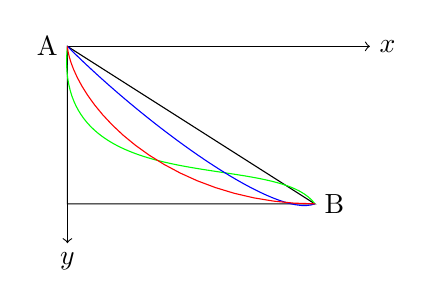
\begin{tikzpicture}
		\node[above,left](A) at (0,0) {A};
		\node[below,right](B) at (pi,-2){B};
		\node[right](x) at (pi + 0.7,0){$x$};
		\node[below](y) at (0,-2-0.5){$y$};
		\draw[->] (0,0) -- (pi + 0.7,0);
		\draw[->] (0,0) --(0,-2-0.5);
		\draw (0,0) -- (0,-2) -- (pi,-2) -- cycle;
		\draw[green] (0,0) .. controls (-0.2,-2) and (pi-0.5,-1.3)  .. (pi,-2);
		\draw[blue] (0,0) .. controls (1,-1) and (pi-0.5,-2.2)  .. (pi,-2);
		\draw[red] plot[domain=0:pi] ({\x - sin(\x r)},{-1 + cos(\x r)});
	\end{tikzpicture}
	\caption{哪个是最速降线?}
\end{figure}

所需总时间:
\[T = \int_{A}^{B} \mathrm{d}T = \int_{A}^{B} \frac{\mathrm{d}L}{v} = \int_{A}^{B} \frac{\sqrt{\mathrm{d}x^2+\mathrm{d}y^2}}{\sqrt{2gy}} = \int_{A}^{B} \frac{\sqrt{1+y'^2}}{\sqrt{2gy}}\mathrm{d}x\]
抽象$\Rightarrow$:
\begin{equation}
S = \int L(f(x),f'(x),x)\mathrm{d}x
\end{equation}
待求函数$f(x)$,使得$S$取极值。数学上这种函数叫做泛函。

\subsection{Euler-Lagrange方程}
求以下泛函的极值:
\begin{equation}
S = \int_{x_1}^{x_2} L(f(x),f'(x))\mathrm{d}x
\end{equation}
函数极值问题启示我们应该在极值函数上尝试做微小改变。

目标极值函数$f_0(x)$,微小改变$|\delta(x)|\ll1$,其中微小改变$\delta(x) = \epsilon \eta(x),\epsilon\rightarrow0$且$\eta(x)$为任意函数。又在端点处应满足:$\delta(x_1) = \delta(x_2) = 0$,所以$\eta(x_1) = \eta (x_2) = 0$,此时有:
\begin{equation}
S = \int_{x_1}^{x_2}L(f,f')\mathrm{d}x \ge S' = \int_{x_1}^{x_2}L(f+\epsilon\eta,f'+\epsilon\eta')\mathrm{d}x
\end{equation}
可将$S$看作$\epsilon$的函数$S(\epsilon)$,在$\epsilon=0$时取极值。即:
\begin{align*}
S'(\epsilon) &= 0\\
             &= \int_{x_1}^{x_2} \left[ \frac{\partial L}{\partial(f+\epsilon\eta)} \cdot \frac{\partial(f+\epsilon\eta)}{\partial\epsilon} + \frac{\partial L}{\partial(f'+\epsilon\eta')} \cdot \frac{\partial(f'+\epsilon\eta')}{\epsilon} \right] \mathrm{d}x\\
             &= \int_{x_1}^{x_2} \left( \frac{\partial L}{\partial f} \cdot \eta + \frac{\partial L}{\partial f'} \cdot \eta' \right)\mathrm{d}x\\
             &= \int_{x_1}^{x_2}  \frac{\partial L}{\partial f} \cdot \eta \mathrm{d}x + \left. \frac{\partial L}{f'} \cdot \eta \right|_{x_1}^{x_2} - \int_{x_1}^{x_2} \left(\frac{\partial L}{f'}\right)'\cdot \eta \mathrm{d}x\\
             &= \int_{x_1}^{x_2} \left[ \frac{\partial L}{\partial f} - \left(\frac{\partial L}{\partial f'}\right)' \right] \cdot \eta \mathrm{d}x = 0
\end{align*}
因为$\eta(x)$是任意函数,所以:
\begin{equation}
\frac{\partial L}{\partial f} - \frac{\mathrm{d}}{\mathrm{d}x}\left(\frac{\partial L}{\partial f'}\right) = 0
\end{equation}
此即Euler-Lagrange方程。

\[S = \int L \mathrm{d}t\]
$S$:作用量(Action),$L$:拉格朗日量(Lagrangian)

!!!!!为何要求在端点处应满足:$\delta(x_1) = \delta(x_2) = 0$,即$\eta(x_1) = \eta (x_2) = 0$!!!!!

\subsection{路径积分的权重因子}

粒子从A到B有多个路径,对每个路径有相应的作用量$S$,每个作用量赋予其一个权重因子:
\[e^{i\frac{S}{\hbar}}\]
对所有路径求和:
\[\sum_{\text{所有路径}}e^{i\frac{S}{\hbar}}\]
此即路径积分因子。<态和态之间的投影因子。>

\subsection{E-L方程应用举例}

\begin{enumerate}
	\item 
		证明:两点间直线最短。
		
		证明:任意两点间距离:
		\[\Delta L^2 = \Delta x^2 + \Delta y^2\]
		作用量为:
		\[S = \int_{A}^{B} \mathrm{d}L = \int_{A}^{B} \sqrt{\mathrm{d}x^2+\mathrm{d}y^2} = \int_{x_A}^{x_B} \sqrt{1 + y'^2} \mathrm{d}x\]
		代入E-L方程:
		\[\frac{\mathrm{d}}{\mathrm{d}x} \left( \frac{\partial \sqrt{1 + y'^2}}{\partial y'} \right) = 0\]
		所以:
		\[\frac{y'}{\sqrt{1 + y'^2}} = C_1 \]
		即:
		\[y' = constant\]
		此即两点间直线最短。\\
	\item
		最小用料问题:优化圆台的侧面使得其侧面面积最小。如图。
		\begin{figure}
			\centering
			\subfigure{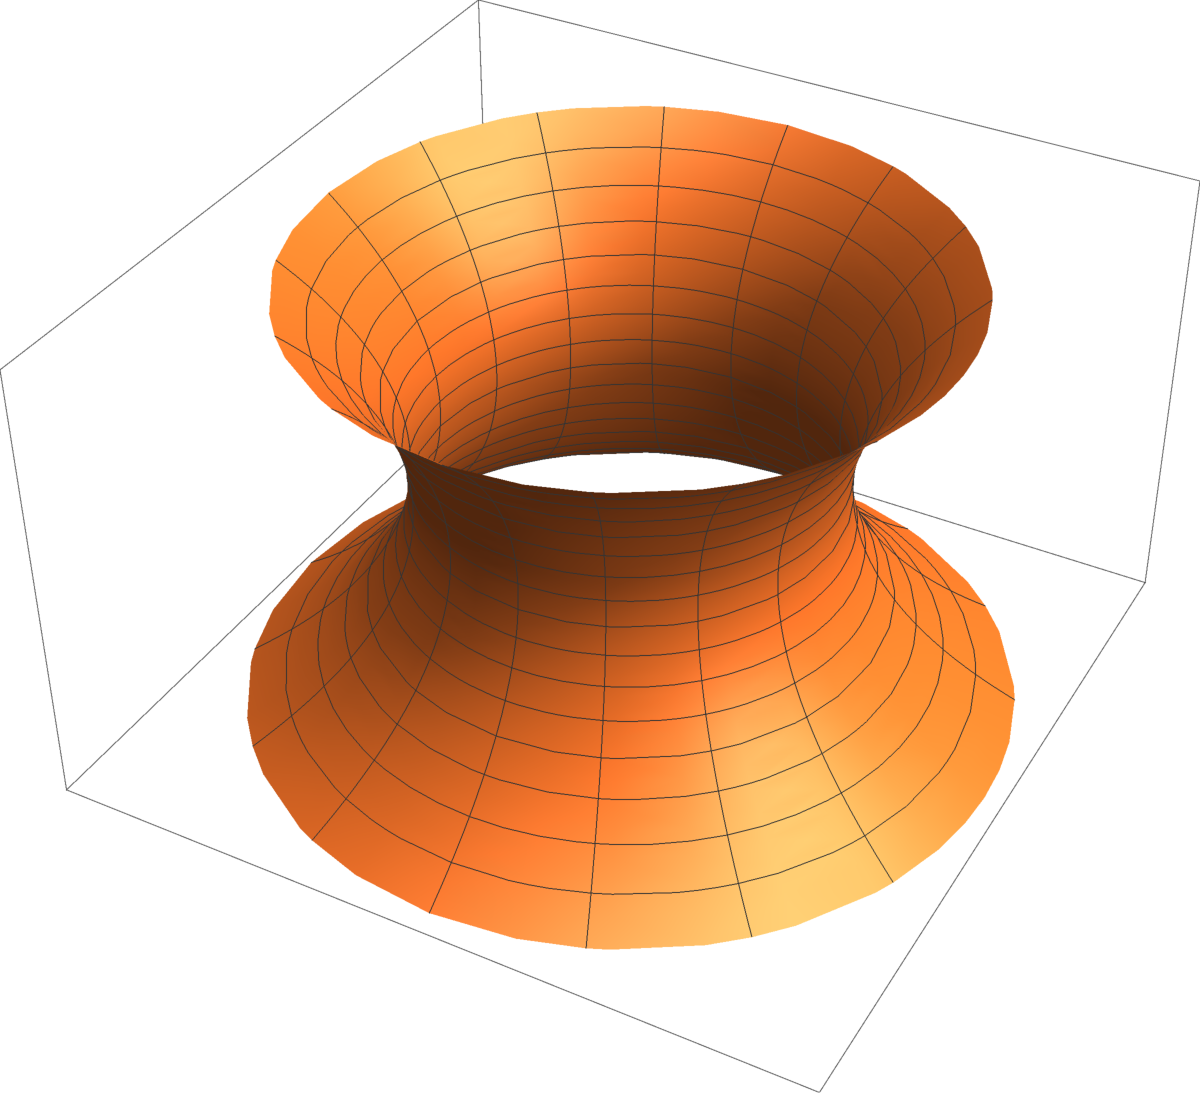
\includegraphics[width=6cm]{Figures/chimney.pdf}}
			\subfigure{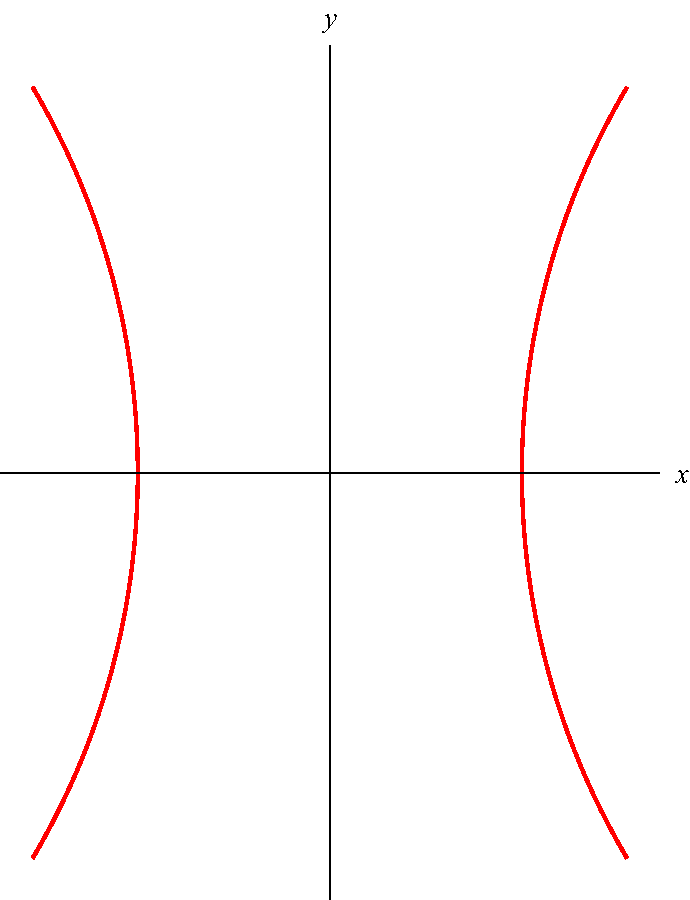
\includegraphics[width=4.7cm]{Figures/chimneysol.pdf}}
			\caption{最小用料问题}
		\end{figure}
		其作用量为:
		\[S = \int_{r_1}^{r_2} 2\pi \sqrt{1+y'^2}\mathrm{d}x\]
		代入E-L方程可得:
		\[\frac{\mathrm{d}}{\mathrm{d}x} \left( \frac{2\pi x y'}{\sqrt{1+y'^2}} \right) = 0\]
		所以:
		\[\frac{x y'}{\sqrt{1+y'^2}} = C_1\]
		即:
		\[y' = \frac{C_1}{\sqrt{x^2-C_1^2}}\]
		所以可以解得:
		\begin{equation}
		\left\{
		\begin{array}{c}
		y = \mathrm{arccosh} \frac{x}{C_1} + C_2\\
		x= C_1 \cosh (y-C_2) 
		\end{array}
		\right.
		\end{equation}
		
		由端点可以确定$C_1,C_2$。
	\item
		给定$z^2 = 8(x^2+y^2)$求连接其上任意两点A,B的曲线方程。
		
		解:采用柱坐标$(z,r,\theta)$,曲面方程变为:$z=8r^2$,曲面上微元的长度:
		\[\mathrm{d}l^2 = 9\mathrm{d}r^2+r^2\mathrm{d}\theta^2\]
		曲线长度:
		\[L = \int_{A}^{B} \mathrm{d}L = \int_{A}^{B}\sqrt{9\mathrm{d}r^2+r^2\mathrm{d}\theta^2} = \int_{A}^{B}\sqrt{9+r^2\theta'^2}\mathrm{d}r\]
		代入E-L方程:
		\[\frac{\mathrm{d}}{\mathrm{d}\theta}\left( \frac{\partial L}{\partial \theta'} \right) = \frac{\mathrm{d}}{\mathrm{d}\theta}\left( \frac{r^2\theta'}{\sqrt{9+r^2\theta'^2}} \right) =0\]
		所以:
		\[\frac{r^2\theta'}{\sqrt{9+r^2\theta'^2}} = k\]
		所以:
		\[\theta' = \frac{3k}{r\sqrt{r^2-k^2}}\]
		所以:
		\begin{equation}
		\left\{
		\begin{array}{c}
		r\cos \left(\frac{\theta+\alpha}{3}\right) = k\\
		z = 2\sqrt{2}r
		\end{array}
		\right.
		\end{equation}
		其中$\alpha,k$为待定常数。
\end{enumerate}

\subsection{理论力学框架}

\begin{tikzpicture}
	\node[above](A) at (0,0) {极值问题};
	\node[below,left](B) at (-1,-1){E-L方程} ;
	\node[below,right](C) at (1,-1) {牛顿力学,量子力学...};
	\draw[<->] (A) -- (B);
	\draw[<->] (B) -- (C);
	\draw[<->] (C) -- (A);
\end{tikzpicture}

\subsubsection{改造牛顿第二定律}

















	%\appendix
	%\include{appendix}
	
	\backmatter%%%%%%%%%%%%%%%%%%%%%%%%%%%%%%%%%%%%%%%%%%%%%%%%%%%%%%%

	%%%%%%%%%%%%%%%%%%%%%%%%%%%%%%%%%%%%%%%%%%%%%%%%%%%%%%%%%%%%%%%%%%%%%%
% 
% This .tex file is coding in utf-8
% 
%%%%%%%%%%%%%%%%%%%%%%%%%%%%%%%%%%%%%%%%%%%%%%%%%%%%%%%%%%%%%%%%%%%%%%
	\printindex
	
	%%%%%%%%%%%%%%%%%%%%%%%%%%%%%%%%%%%%%%%%%%%%%%%%%%%%%%%%%%%%%%%%%%
	
\end{document}